\documentclass[a4paper, 16pt]{article}
\usepackage[T1]{fontenc}
\usepackage{hyperref}
\usepackage[all]{hypcap}
\usepackage[utf8]{inputenc}
\usepackage{graphicx}
\usepackage[left=2cm, top=3cm, text={17cm, 24cm}]{geometry}
\usepackage[czech, english]{babel}
\selectlanguage{english}
\usepackage{subfig}
\usepackage{color}
\usepackage{url}
\inputencoding{utf8}
\usepackage{float}
\usepackage{hyperref}
\usepackage[all]{hypcap}
\hypersetup{colorlinks=false, linkbordercolor=1 1 1, citebordercolor=1 1 1}
\usepackage[right]{lineno}
\renewcommand\linenumberfont{\normalfont\tiny\color{blue}}


\author{Ondrej Valo, \href{mailto:xvaloo00@stud.fit.vutbr.cz}{xvaloo00@stud.fit.vutbr.cz}\\
Radoslav Páleník, \href{mailto:xpalen05@stud.fit.vutbr.cz}{xpalen05@stud.fit.vutbr.cz}\\
Karel Fritz, \href{mailto:xfritz00@stud.fit.vutbr.cz}{xfritz00@stud.fit.vutbr.cz}
}
\title{Projektová dokumentácia UPA }
\date{zima 2022}

\begin{document}
\maketitle

\section{Exploratívna analýza}

\subsection{Atributy datové sady}
Dataset obsahuje celkovo 344 záznamov s atribútmi, ktoré jemožné rozdeliť na 2 podmnožiny:

\subsubsection{Atribúty odberu}
\begin{itemize}
    \item \textbf{studyName} [\emph{string}]\\
    Štúdia z ktorej pochádza odber. V datasete sú záznamy zo štúdií \emph{PAL0708}, \emph{PAL0809} a \emph{PAL0910}.
    \item \textbf{Sample Number} [\emph{int}]\\
    Číslo vzorky odberu. Jednotlivé vzorky sú číslované chronologicky v poradí odberov.
   
    \item \textbf{Region} [\emph{string}]\\
    Región merania. Všetky zaznamenané odbery prebehli v regióne Anvers.
     
    \item \textbf{Island} [\emph{string}]\\
    Ostrov Palmerského súostrovia. Definuje ostrov, na ktorom bol daný odber uskutočnený. V datasete sa nachádzajú celkovo 3 ostrovy: \emph{Torgersen}, \emph{Biscoe} a \emph{Dream}. Najpočetnejšie zastúpenie v meraniach má ostrov \emph{Biscoe} s celkovým podielom 49\%.
\end{itemize}

\subsubsection{Atribúty sledovaného tučniaka}
\begin{itemize}
     \item \textbf{Species} [\emph{string}]\\
    Druh tučniaka. Dataset sleduje merania na troch druhoch tučniakov: \emph{Adelie}, \emph{Chinstrap} a \emph{Gentoo}. Najpočetnejším druhovým zástupcom v záznamoch je \emph{Adelie} s podielom  44\% vo všetkých výskytoch.
    \item \textbf{Stage} [\emph{string}]\\
    Reprodukčné štádium počas odberu. Pre tento atribút sa v datasete objavuje len 1 hodnota, \uv{Adult, 1 Egg Stage}. Dataset teda uvažuje jedno vajce v každej znáške.
    
    \item \textbf{Individual ID} [\emph{string}]\\
    Unikátny identifikátor študovaného tučniaka. Celkovo sa v datasete nachádza 190 unikátnych jedincov.
    
    \item\textbf{ Clutch Completion} [\emph{bool}]\\
    Dokončenie znášky. Počas meraní sa sleduje, či v čase merania bol splodený nový jedinec. V datasete sa nachádza 89.5\% záznamov s hodnotou \emph{true}.
    
    \item \textbf{Date Egg} [\emph{date}]\\
    Dátum odberu vzorky. Zaznamenané odbery prebehli v rozmedzí od 9.11.2007 do  1.12.2009.
    
    \item \textbf{Sex} [\emph{string}]\\
    Pohlavie tučniaka, v datasete sa uvádzajú 2 rôzne hodnoty: \emph{FEMALE} a \emph{MALE}. 
    
    \item \textbf{Culmen Length (mm)} [\emph{float}]\\
    Dĺžka vrchnej časti zobáku (v \emph{mm})
    
    \begin{table}[H]
    \centering
    \begin{tabular}{|c|c|c|}
    \hline
    \textbf{Minimum} & \textbf{Priemer} & \textbf{Maximum} \\ \hline
             32.1             &     43.92             &   59.6                    \\ \hline
    \end{tabular}
    \end{table}
    
    \item \textbf{Culmen Depth (mm)} [\emph{float}]\\
    Hĺbka vrchnej časti zobáku (v \emph{mm})
    \begin{table}[H]
        \centering
        \begin{tabular}{|c|c|c|}
        \hline
        \textbf{Minimum} & \textbf{Priemer} & \textbf{Maximum} \\ \hline
                          13.1    &      17.15            &   21.5                    \\ \hline
        \end{tabular}
    \end{table}
    
    \begin{figure}[H]
    \centering
    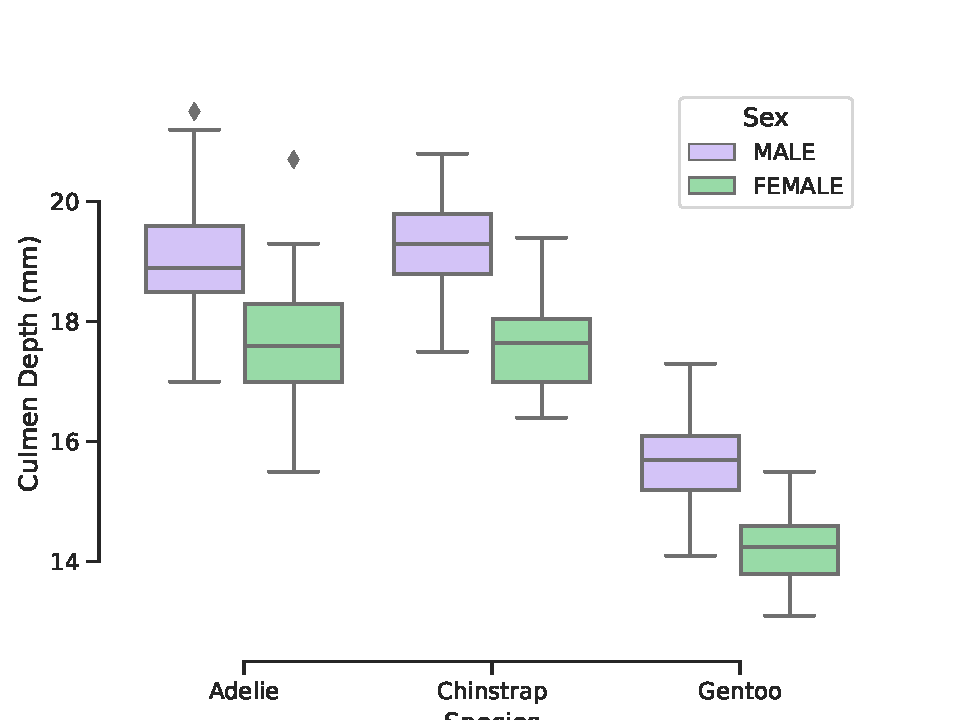
\includegraphics[width=15cm]{graphs/culmen_d.pdf}
    \caption{Distribúcia hĺbky vrchnej časti zobáku}
    \label{fig:2}
    \end{figure}
    
    
    \newpage
    
    
    \item \textbf{Flipper Length (mm)} [\emph{float}]\\
    Dĺžka plutvy (v \emph{mm})
    \begin{table}[H]
    \centering
    \begin{tabular}{|c|c|c|}
    \hline
    \textbf{Minimum} & \textbf{Priemer} & \textbf{Maximum} \\ \hline
                  172        &        200.92          &  231                     \\ \hline
    \end{tabular}
    \end{table}
    
    \begin{figure}[H]
    \centering
    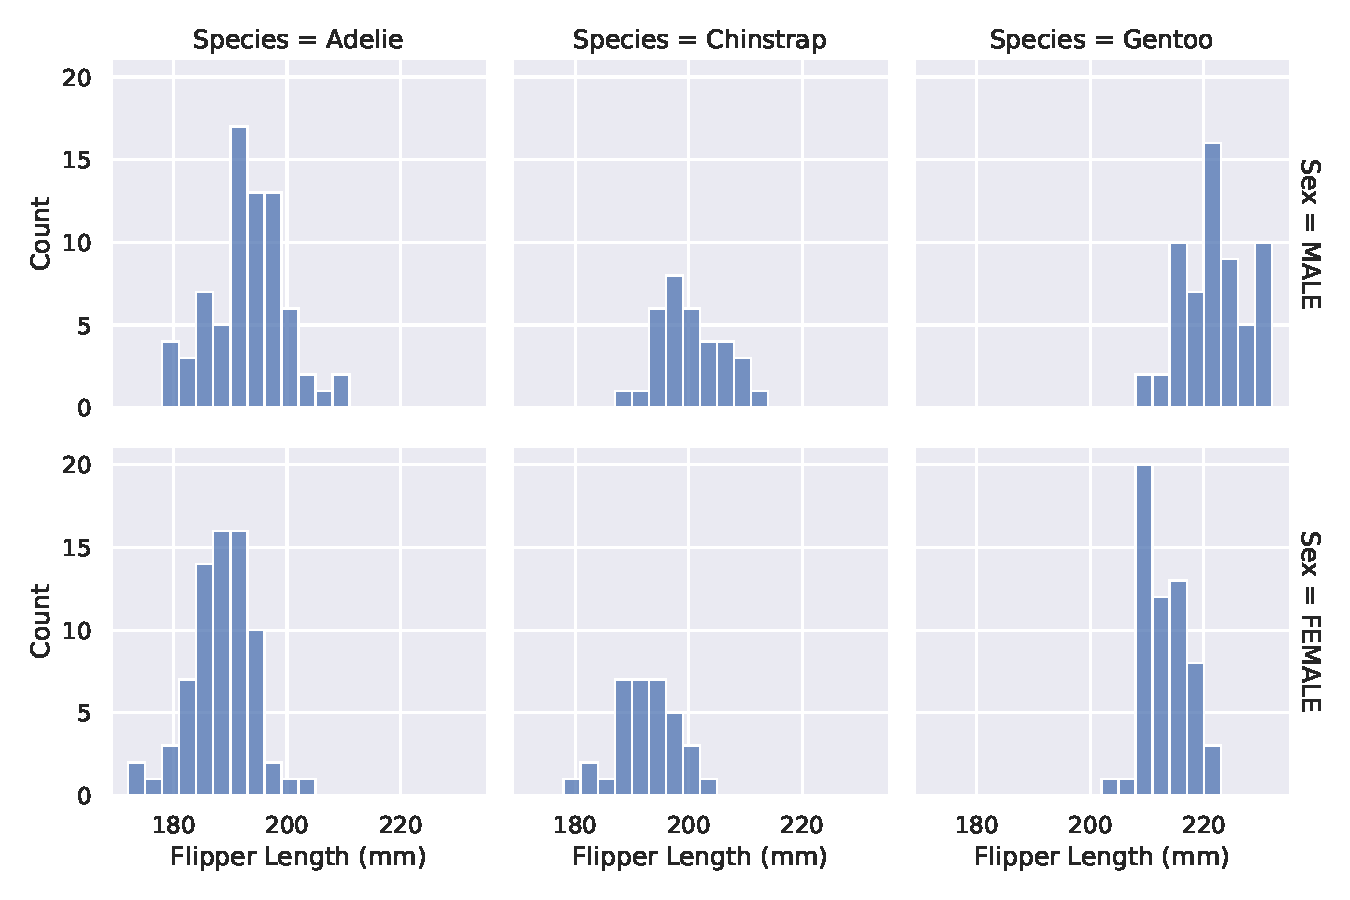
\includegraphics[width=15cm]{graphs/flipper_l.pdf}
    \caption{Distribúcia dĺžky plutiev}
    \label{fig:3}
    \end{figure}
    
     \item \textbf{Delta 15 N (o/oo)} [\emph{float}]\\
    Miera pomeru stabilných izotopov 15N:14N
    \begin{table}[H]
    \centering
    \begin{tabular}{|c|c|c|}
    \hline
    \textbf{Minimum} & \textbf{Priemer} & \textbf{Maximum} \\ \hline
                7.63          &       8.73         & 10.03                     \\ \hline
    \end{tabular}
    \end{table}
    \item \textbf{Delta 13 C (o/oo)} [\emph{float}]\\
    Miera pomeru stabilných izotopov 13C:12C
    \begin{table}[H]
    \centering
    \begin{tabular}{|c|c|c|}
    \hline
    \textbf{Minimum} & \textbf{Priemer} & \textbf{Maximum} \\ \hline
               -27.02           &  -25.69         &   -23.79                    \\ \hline
    \end{tabular}
    \end{table}
    
    
    
    \newpage
    
    
    \item \textbf{Body Mass (g)} [\emph{float}]\\
    Telesná  masa tučniaka (v \emph{g})
    \begin{table}[H]
    \centering
    \begin{tabular}{|c|c|c|}
    \hline
    \textbf{Minimum} & \textbf{Priemer} & \textbf{Maximum} \\ \hline
                 2700         &       4201.75           &    6300                   \\ \hline
    \end{tabular}
    \end{table}
    
    \begin{figure}[H]
    \centering
    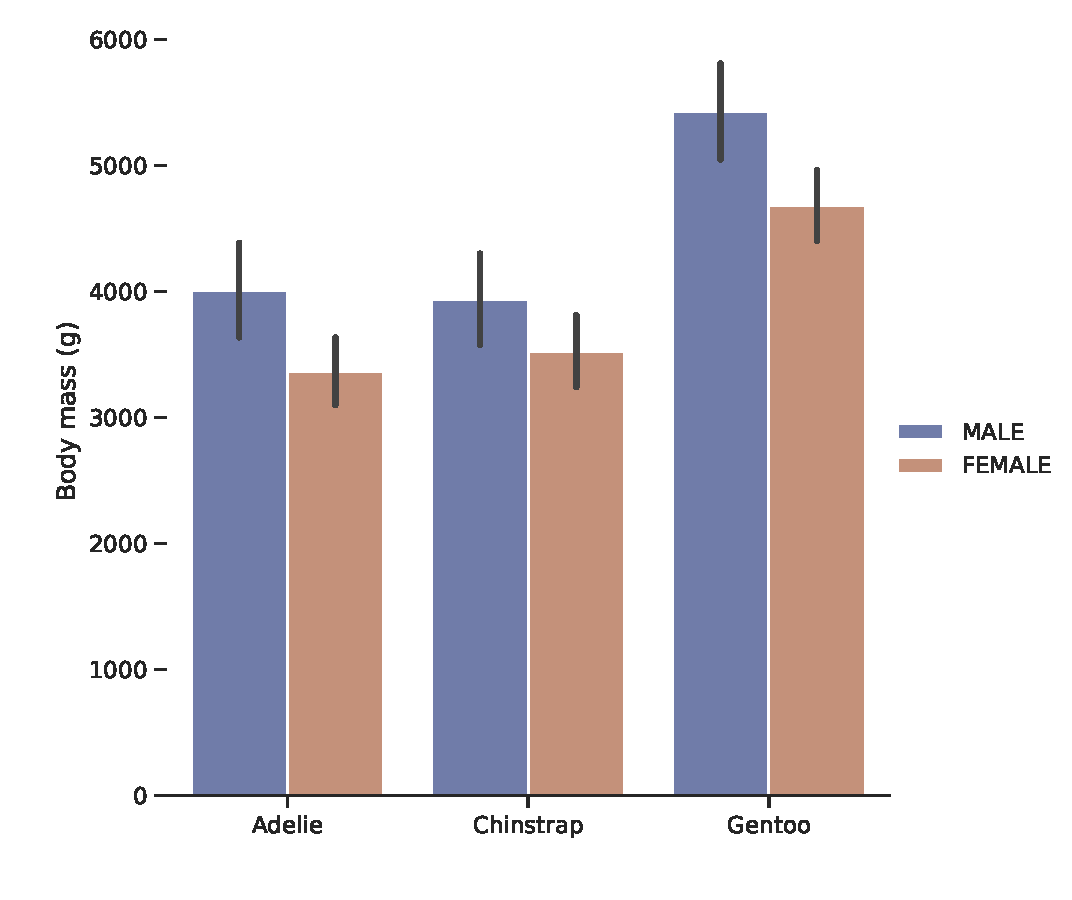
\includegraphics[width=15cm]{graphs/weight.pdf}
    \caption{Distribúcia telesnej masy tučniakov}
    \label{fig:4}
    \end{figure}
   
  
  
    
    \item\textbf{Comments} [\emph{string}]\\
    Komentár k meraniu určený na obsiahnutie iných relevantných informácií k dátam.

\end{itemize}
\newpage
\subsection{Analýza chýbajúcich hodnôt}
V databáze sa celkovo nachádza 12 záznamov s 2 a viac chýbajúcimi atribútmi. Majoritu chýbajúcich atribútov tvorí atribút \emph{Comments} (chýba v 318 záznamoch). Tento atribút sa totiž využíva najmä ako poznámka pri nekompletných záznamoch, príp. pri záznamoch jedincov u ktorých nebola počas skúmania zaznamenaná znáška. Okrem komentárov je početnosť chýbajúcich  atribútov nasledovná: 


    \begin{table}[H]
    \centering
    \begin{tabular}{|c|c|c|}
    \hline
    \textbf{Atribút} & \textbf{Počet}& \textbf{Najčastejšie odôvodnenie}\\ \hline
     Delta 15 N (o/oo)  &     14 &    Nedostatok krvi na testy \\ \hline
      Delta 13 C (o/oo)&      13 &     Nedostatok krvi na testy\\ \hline
      Sex&        11   &  Nedostatok krvi na testy\\ \hline
      Culmen Length (mm)&      2 &   Jedinec nebol meraný \\ \hline
      Culmen Depth (mm)&    2   &    Jedinec nebol meraný\\ \hline
      Flipper Length (mm)&  2   &    Jedinec nebol meraný  \\ \hline
      Body Mass (g)&       2  &  Jedinec nebol meraný\\ \hline
    \end{tabular}

\end{table}

\subsection{Korelačná analýza numerických atribútov}

\begin{figure}[H]
    \centering
    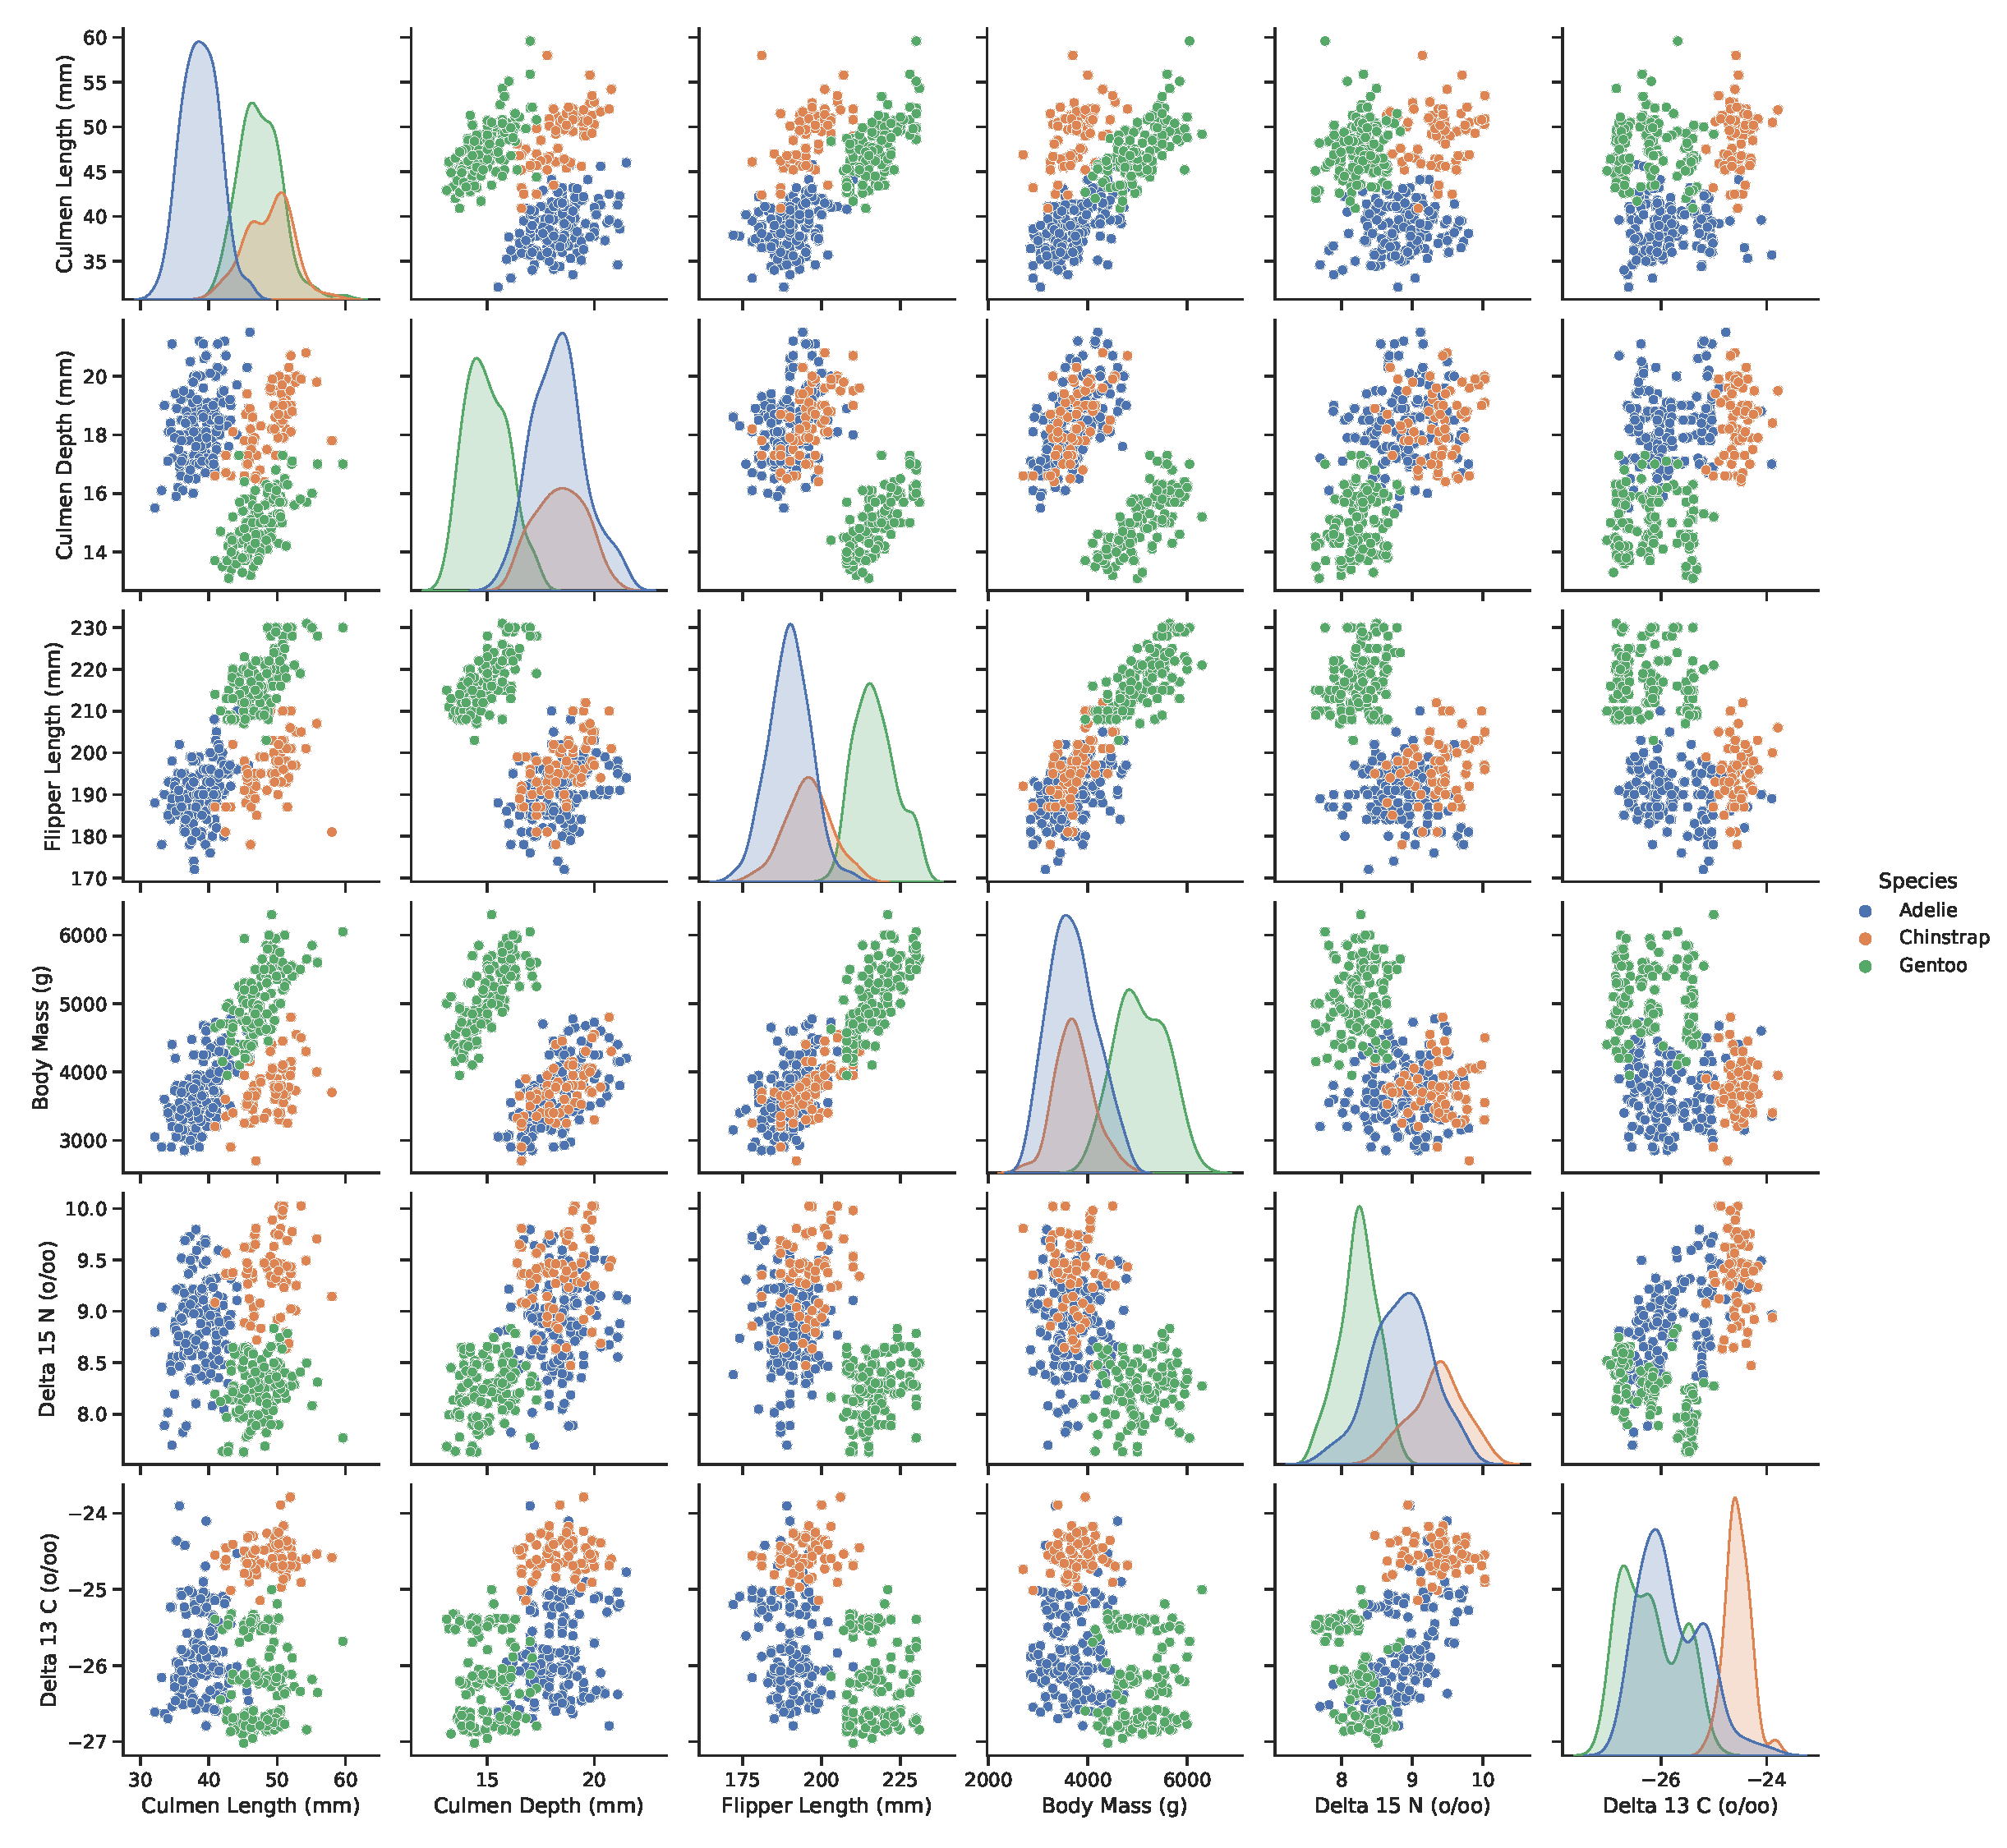
\includegraphics[width=15cm]{graphs/corelation_a.pdf}
    \caption{Korelácia dát medzi všetkými numerickými atribútami}
    \label{fig:5}
\end{figure}
Z grafov \ref{fig:5} môžeme pozorovať nenulovú koreláciu skoro pre všetky numerické atribúty danej dátovej sady. Aj keď je možno vidieť vyšiu koreláciu medzi niektorými atribútami ako je dĺžka krídiel a dĺžka hrany zobáka, oproti nižším ako je hmotnosť s hĺbkou zobáka pre druhy Adelie a Chinstrap. Koreláciu v nie veľmi očakávaných atribútoch si môžeme vysvetliť, vysokým rozdielom v daných atribútov medzi druhmi ča nám ukazujú grafy po diagonále obrázku.

\begin{figure}[H]
    \centering
    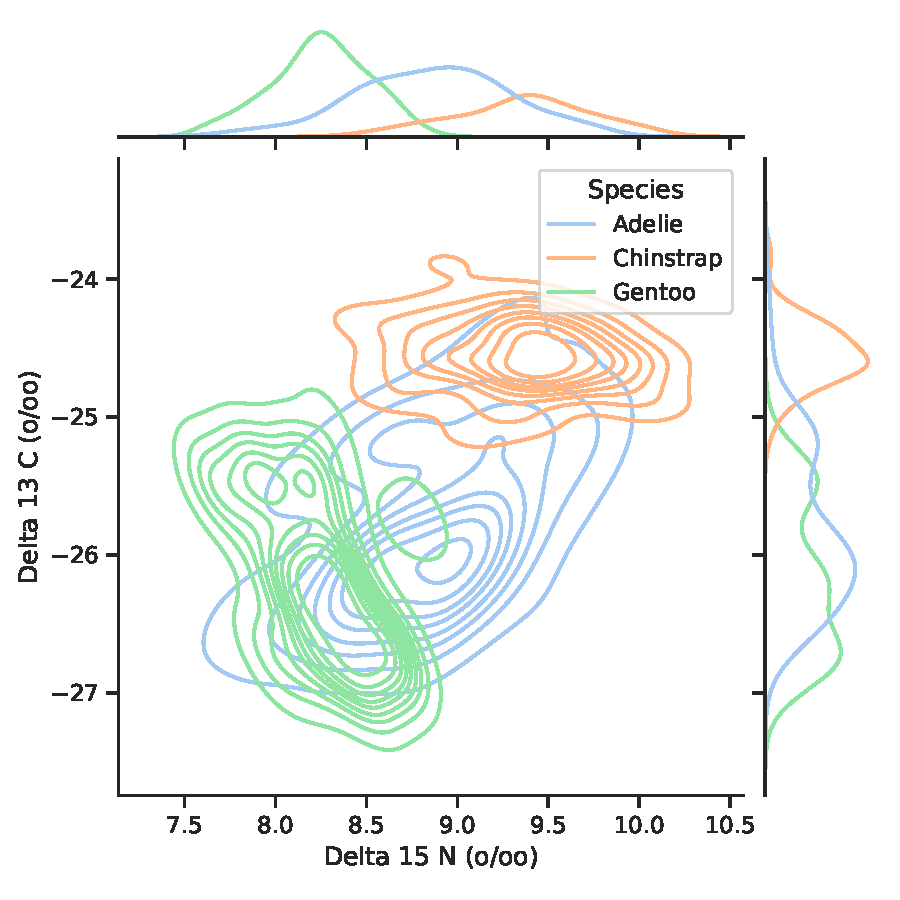
\includegraphics[width=15cm]{graphs/isotopes_N_C.pdf}
    \caption{Korelácia izotopov v krvi}
    \label{fig:6}
\end{figure}
Z grafu \ref{fig:6} môžeme vyčítať nižší počet izotopov Typu C a N pre tučniaky druhu Gentoo, a vyšší pre Chinstrap.
Tučniaky Adelie majú väčší rozsah počtu izotopov.

\begin{figure}[H]
    \centering
    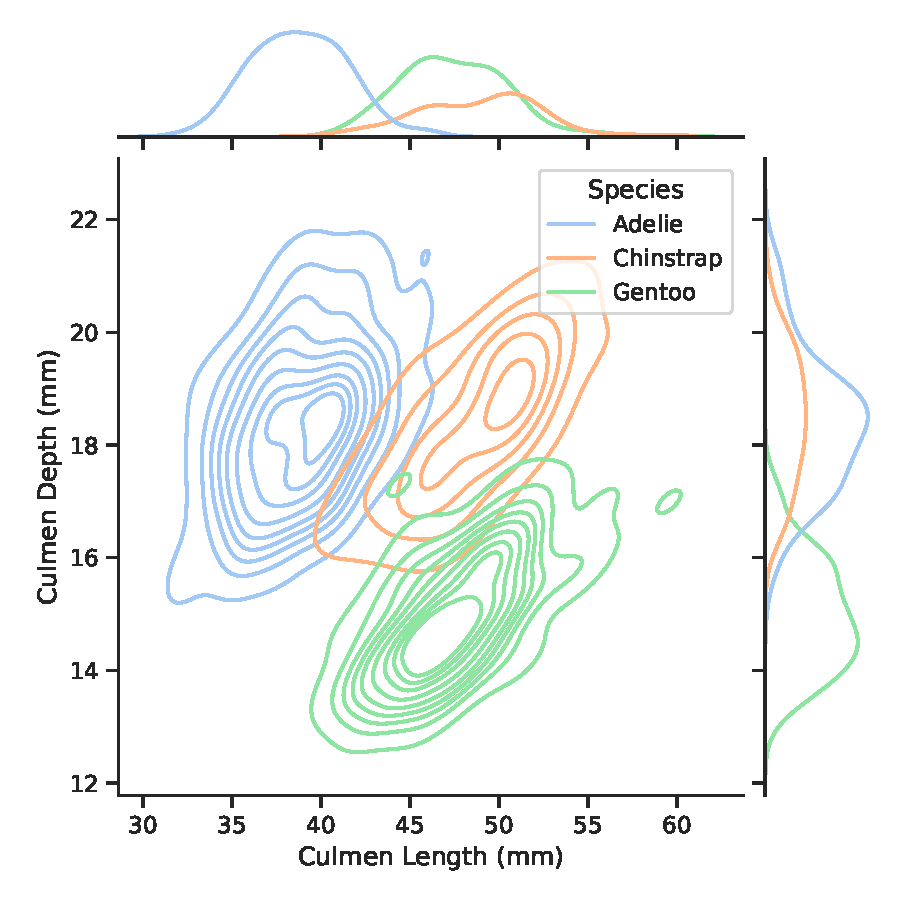
\includegraphics[width=15cm]{graphs/culmen_l_d.pdf}
    \caption{Korelácia vrchnej časti zobáku}
    \label{fig:7}
\end{figure}
Z grafu \ref{fig:7} môžeme vyčítať že tučniaky Adelie majú nižšiu dĺžku ale väčšiu hĺbku hrany zobáka, Gentoo sú presný opak a Chinstrap majú rovnomerne dlhú a hlbokú hranu zobáku.

\section{Príprava dátovej sady pre dolovacie algoritmy}
Prvým dôležitým krokom je odstrániť nerelevantné informácie. Jedná sa o informácie, ktoré z logického hľadiska neprispievajú k správnej klasifikácii. Ako nerelevantné môžeme považovať informácie zo stĺpcov \uv{studyName, Sample Number, Region, Stage, Individual ID, Clutch Completion, Date Egg, Comments}. Keďže ani jeden z týchto stĺpcov nie je informačne pre klasifikáciu dôležitý, sú tieto stĺpce odstránené.

%Jako první krok bylo důležité odstranit nerelevantní informace, tedy takové jež z logického hlediska nepřispívají ke správné klasifikaci. Tyto informace odpovídají sloupcům 'studyName', 'Sample Number', 'Region', 'Stage', 'Individual ID', 'Clutch Completion', 'Date Egg', 'Comments'. Jelikož ani jeden z těchto sloupců není informačně důležitý pro klasifikaci jsou tyto sloupce odstraněny.


\subsection{Kategorická príprava}
Pri týchto dátach boli pre chýbajúce hodnoty odstránené celé riadky(záznamy). Odstránenie hodnôt bolo prevedené pomocou \emph{DataFrame.dropna()} z knižnice \emph{pandas}. Ďalej sa tu odľahlé hodnoty nevyskytovali, dataset bol vysokej kvality s menším počtom záznamov, mierné vyhladenie hodnôt prebehlo vďaka metóde \emph{qcut()} opäť z knižnice \emph{pandas}. Táto metóda prevedie kvantilovú diskretizáciu, teda rozdelí dáta do n košov tak, aby v každom koši bol rovnaký počet záznamov. Pri uvedenej implementácii sa používa 8 košov. Tým je príprava dát pre klasifikátor pracujúci s kategorickými vstupmi dokončená.

%U těchto dat byly pro chybějící hodnoty odstraněny celé řádky (záznamy). Odstranění hodnot bylo provedeno metodou DataFrame.dropna() z knihovny pandas. Dále odlehlé hodnoty se zde nevyskytovaly, dataset byl vysoké kvality s méně záznamy, mírné vyhlazení odlehlých hodnot proběhlo díky metodě qcut() opět z knihovny pandas. Metoda qcut() provede qvantilovou diskretizaci, tedy rozdělí data do n košů tak aby v každém koši byl stejný počet záznamů. My jsme zvolili 8 jako počet košů. Tím je příprava dat pro klasifikátor pracující s kategorickými vstupy dokončena.


\subsection{Numerická príprava}
U chýbajúcich hodnôt tu bola vykonaná interpolácia, aj pomocou metódy z knižnice \emph{pandas}, konkrétne \emph{DataFrame.interpolate()}. Keďže v dátach neboli žiadne významné odľahlé hodnoty, prešlo sa ihneď k numerifikácii. Metóda \emph{get\_dummies()} funguje na princípe algoritmu one-hot encoding, ktoré vytvorí z kategorických hodnôt numerické. Naviac zachová rovnakú dôležitosť vďaka zakódovaniu iba pomocou 0 a 1, teda pokiaľ bol tučniak samec, budú hodnoty pre stĺpce priradené následovne: Gender-male 1 a Gender-female 0.

\bigskip
Normalizácia hodnôt prebehla nasledovne: Pre všetky stĺpce sa nahradia ich hodnoty novou hodnotou získanou ako podiel hodnoty v riadku daného stĺpcu s maximálnou hodnotou daného stĺpcu. Tím je dataset pripravený pre klasifikátor využívajúce numerické vstupy.
%
%U chybějících hodnot zde byla provedena interpolace, také pomocí metody z knihony pandas, konkrétně %DataFrame.interpolate(). Jelikož v datech nebyly žádné významné odlehlé hodnoty, přešlo se ihned k %numerifikaci. Metoda get\_dummies() funguje na principu algoritmu one-hot encoding jež vytvoří z %kategorických hodnot hodnoty numerické. Navíc zachová stejnou důležitost díky zakódování pouze %pomocí 1 a 0. Tedy pokud tučňák byl samec, dostane sloupe Gender-male 1 a Gender-female 0, nikoliv %Gender 1 nebo 2 podle toho zda je samec či samice. 
%
%\bigskip
%Normalizace hodnot proběhla následovně: Pro všechny sloupce nahraď hodnoty v nich hodnotou podílu %hodnoty v řádku daného sloupce a maximální hodnotou daného sloupce. Tím je náš dataset připravený %pro klasifikátor využívající numerické vstupy.

\end{document}
